\documentclass[openright, a4paper]{article}
\usepackage{graphicx}
\usepackage{kotex}
\usepackage{minted}
\usepackage{setspace}
\usepackage{underscore}
\usepackage{caption}
\usepackage{array}
\usepackage{multirow}
\usepackage[margin=3cm]{geometry}
\newcommand{\code}[1]{\texttt{#1}}
\setminted{
    linenos=true,
    autogobble,
}
\newenvironment{longlisting}{\captionsetup{type=listing}}{}
\captionsetup{labelformat=empty,labelsep=none}

\title{2024학년도 컴퓨터구조 Lab Assignment \#4-1\\
        Pipelined CPU w/o control flow instructions}

\author{김도영, 선민수}
\date{2024년 4월 30일}

\onehalfspacing
\begin{document}

\maketitle

%%%%%%%%%%%%%%%%%%%%%%%%%%%%%%%%%%%%%%%%%%%%%%%%%%%%%
%                   Introduction                    %
%%%%%%%%%%%%%%%%%%%%%%%%%%%%%%%%%%%%%%%%%%%%%%%%%%%%%

\section{Introduction}
이 과제에서는 Verilog를 이용하여 이전 과제인 Multi Cycle CPU를 개선한 Pipelined CPU를 구현하는 것을 목적으로 한다. Pipelined CPU의 가장 큰 차이점은 기존 Single Cycle CPU나 Multi Cycle CPU의 경우 동시에 하나의 instruction만을 처리할 수 있었지만, Pipelined CPU는 Pipelining을 통하여 동시에 최대 5개의 instruction을 실행할 수 있는 점이다. 기존의 Multi Cycle CPU 대비 장점은 다음과 같다.

\begin{itemize}
    \item Multi Cycle CPU에서도 개선되지 못하였던, Instruction 실행 시 모듈들이 작동하지 않고 유휴 상태로 낭비되는 것을 Pipelining을 통하여 막았고 효율적으로 사용한다.
    \item Multi Cycle CPU까지도 한 개의 Instruction이 끝나기 전까지는 이전의 Instruction이 절대 실행 혹은 처리되지 않았지만, Pipelining을 통해서 각 스테이지별 Instruction을 사용하여 Instruction의 Throughput을 증가시켰다.
\end{itemize}

%%%%%%%%%%%%%%%%%%%%%%%%%%%%%%%%%%%%%%%%%%%%%%%%%%%%%
%                      Design                       %
%%%%%%%%%%%%%%%%%%%%%%%%%%%%%%%%%%%%%%%%%%%%%%%%%%%%%

\section{Design}
본 과제에서 구현한 Pipelined CPU는 수업 시간에 배운 Data Path와 교과서의 Signal을 기준으로 구현하였으며, 추가적으로 Data Forwarding을 함께 구현하였다.

\hfill

Pipelined CPU는 이전 Multi Cycle CPU와 같이 IF - ID - EX - MEM - WB의 스테이지로 나뉘어서 실행된다. Multi Cycle CPU와의 차이점은 모든 스테이지가 동시에 사용된다는 점으로, Instruction 1이 ID 스테이지에서 처리될 때, 다른 Instruction 2는 IF 스테이지를 거치는 식으로 동시에 최대 5개의 instruction을 처리한다.

\hfill

Data hazard가 발생하는 경우에는 Hazard Detection Module을 통해서 Hazard 발생을 탐지하고 Hazard가 발생된 원인(레지스터의 WB Stage, Store Instruction의 MEM Stage 등)이 모두 완료될 때까지 Stall하여 이를 해결한다.

\hfill

레지스터가 아직 WB되지 않아 발생하는 Hazard는 Data Forwarding을 통하여 WB 이전에 값을 받아와 Stall되는 시간을 줄여, 최적화할 수 있다. 해당 과제에서는 Data Forwarding을 함께 구현한다.

\hfill

구현한 Pipelined CPU는 아래와 같은 구조를 가진다. (단, 그림에서 Data Forwarding Unit과 Hazard Detection Module은 표현되지 않았다.) 구현에서의 \code{wire}나 \code{reg}의 이름은 아래 그림에서 제시된 이름을 사용한다.

\hfill

{
    \begin{figure}[!h]
        \centering
        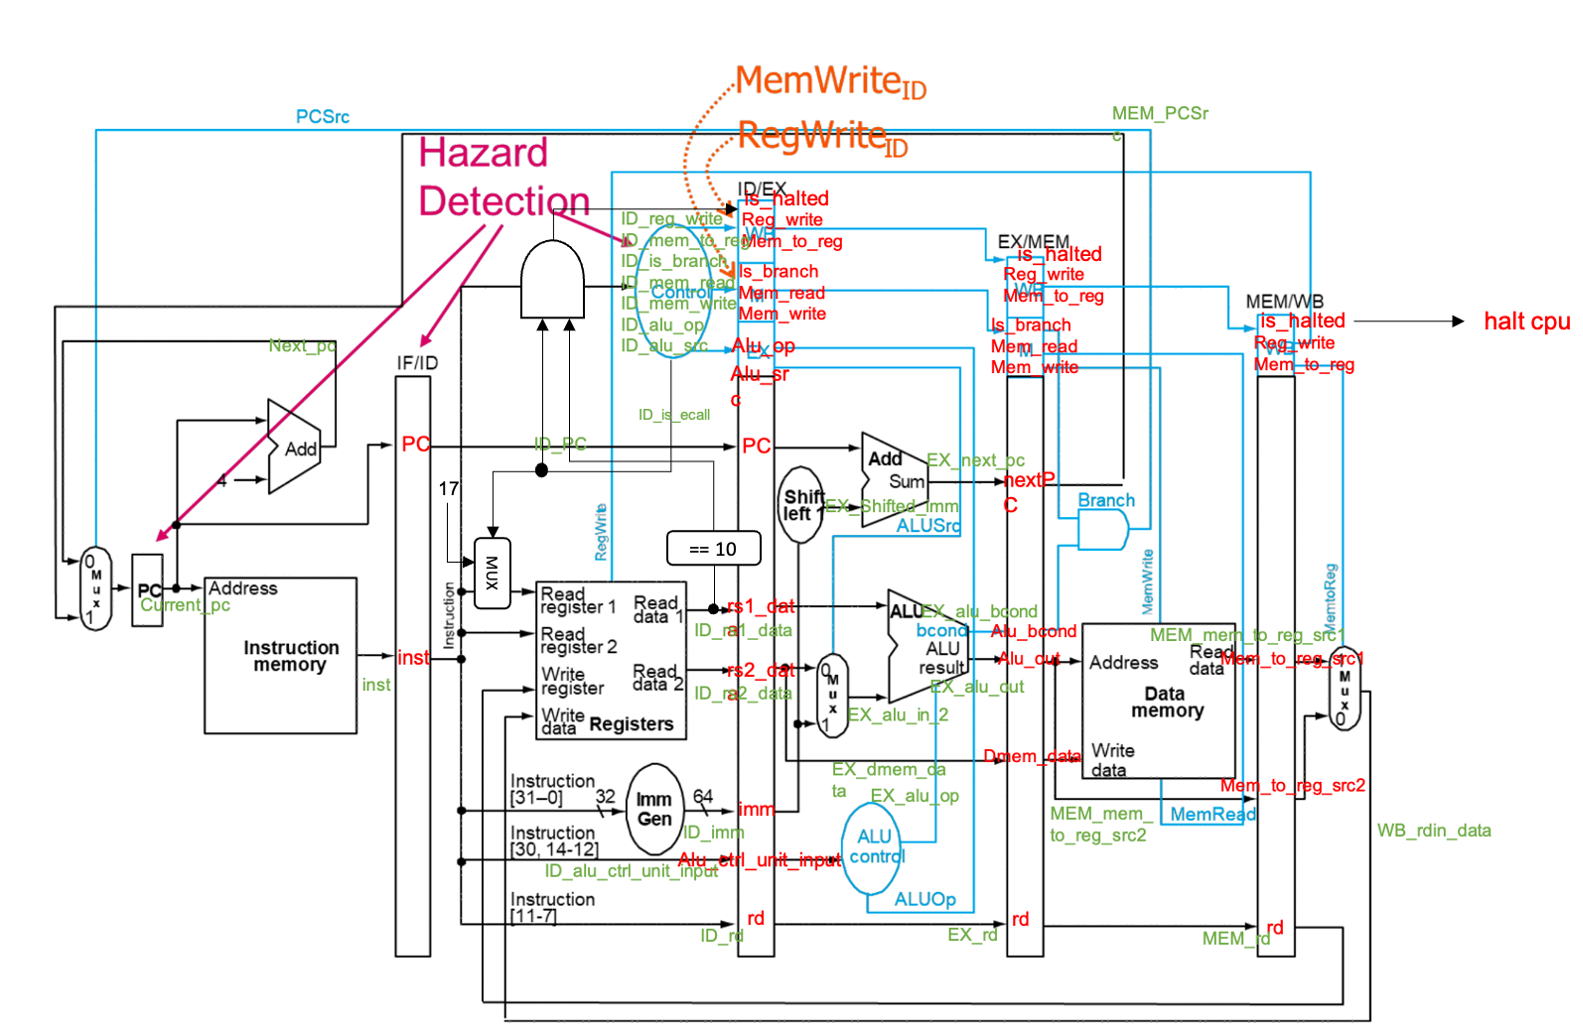
\includegraphics[width=\textwidth]{img/schematic.png}
        \caption{Design of Pipelined CPU}
    \end{figure}
}

\hfill

Pipelined CPU를 구성하는 세부 모듈들과 각각의 역할은 아래와 같다.

\hfill

\begin{itemize}
    \item PC: 현재의 program counter 값을 저장하는 모듈로, clock의 positive 
    edge마다 \code{next_pc} 신호를 받아 \code{pc_write} 신호가 \code{1}일 때 
    program counter를 업데이트하는 동기 회로이다.

    \item Hazard Detection Module: 현재 실행되어야 하는 Instruction이 앞서 실행된 Instruction의 실행 종료를 기다려야 하는지에 대한 여부를 판단하는 모듈이다. 주어진 Instruction에 대해 이전 Instruction의 Dependency를 계산하는 비동기 회로이다.

    \item Forwarding Unit: Stall로 인한 딜레이를 최소화하고자 ALU의 피연산자를 MEM 혹은 WB Stage에서 바로 Fetch할 수 있는지에 대한 여부를 판단하여, MEM 혹은 WB Stage에서의 사용때문에 생기는 Stall을 줄일 수 있는 모듈이다. 주어진 Instruction에 대해 해당 피연산자들이 어느 단계에서 사용되고 있는지를 판단하는 비동기 회로이다.
    
    \item Control: 현재 명령어의 opcode를 받아 명령어의 실행 과정에 따라 
    해당하는 control 신호를 계산하는 비동기 회로이다.
    
    \item Registers: CPU의 programmer visible state 중 하나인 레지스터이다. 
    \code{x0}부터 \code{x31}까지 총 32개를 가지고 있다. Register의 업데이트는 clock의 negative 
    edge에서 업데이트되는 동기 회로이며, Register의 읽기의 경우 비동기 회로이다.

    \item Immediate Generator: 명령어를 받아 명령어에 따른 immediate 값을 계산하는 모듈로, 
    비동기 회로이다.

    \item ALU control: ALU가 수행해야 할 연산을 지정해주는 ALU control 신호를 
    계산하는 비동기 회로 모듈이다.

    \item ALU: 두 입력값과 ALU contorl 신호를 받아 해당하는 연산을 하는 
    모듈로, 입력이 바뀌면 출력도 곧바로 바뀌는 비동기 회로이다.

    \item Memory: 실제 CPU에 연결된 memory의 역할을 하는 모듈로, Instruction Memory와 Data Memory를 구분하여 사용한다. clock의 positive edge마다 입력에 따라 메모리 값을 변경하는 동기 회로이다.

    \item Pipeline Register: 각 Stage 별로 다음 Stage에 넘겨주어야 할 Control Signal이나 Register의 정보 등의 신호를 저장하는 Register이다. 스테이지의 사이마다 존재하여 값을 넘겨준다. Clock의 Positive Edge마다 Stage에서 계산된 결과를 Fetch하여 Register의 값을 변경하는 동기 회로이다.
\end{itemize}

%%%%%%%%%%%%%%%%%%%%%%%%%%%%%%%%%%%%%%%%%%%%%%%%%%%%%
%                 Implementation                    %
%%%%%%%%%%%%%%%%%%%%%%%%%%%%%%%%%%%%%%%%%%%%%%%%%%%%%

\section{Implementation}

\subsection{Program Counter}

\begin{figure}[h]
\begin{longlisting}
    \begin{minted}[fontsize=\footnotesize]{Verilog}
always @(posedge clk) begin
    if(reset) 
        current_pc <= 0;
    else if(pc_write)
        current_pc <= next_pc;
end
    \end{minted}    
    \caption{PC.v}
\end{longlisting}
\end{figure}

Program Counter는 주어진 clk에 따라서 current_pc를 next_pc로 업데이트하는 Synchronous 모듈이다. \\

\subsection{Control Unit}

\begin{longlisting}
    \begin{minted}[fontsize=\footnotesize]{Verilog}
always @(*) begin
    mem_read = (opcode == `LOAD);
    mem_to_reg = (opcode == `LOAD);
    mem_write = (opcode == `STORE) && (!is_hazard);
    alu_src = (opcode != `ARITHMETIC) && (opcode != `BRANCH);
    write_enable = (opcode != `STORE) && (opcode != `BRANCH) && (!is_hazard);
    alu_op = {
        (opcode == `ARITHMETIC) || 
        (opcode == `ARITHMETIC_IMM) || 
        (opcode == `BRANCH),
        1'b0
    };
    is_ecall = (opcode == `ECALL);
end
    \end{minted}
    \caption{ControlUnit.v}
\end{longlisting}

Control Unit은 주어진 instruction에서 opcode에 따라 필요한 Control Value를 계산하여 산출하는 Asynchronous 모듈이다. \\

\subsection{ALU Control Unit}

\begin{longlisting}
    \begin{minted}[fontsize=\footnotesize]{Verilog}
always @(*) begin
    case(aluOp)
        2'b00: alu_op = `ALU_ADD;
        2'b01: alu_op = `ALU_SUB;
        default: begin
            case(instruction[6:0])
                `ARITHMETIC: begin
                    case(instruction[14:12])
                        `FUNCT3_ADD: alu_op = (instruction[30]) ? `ALU_SUB : `ALU_ADD;
                        `FUNCT3_SLL: alu_op = `ALU_SLL;
                        `FUNCT3_SRL: alu_op = `ALU_SLR;
                        `FUNCT3_AND: alu_op = `ALU_AND;
                        `FUNCT3_OR:  alu_op = `ALU_OR;
                        `FUNCT3_XOR: alu_op = `ALU_XOR;
                        default:     alu_op = 4'b0;
                    endcase
                end
                `ARITHMETIC_IMM: begin
                    case(instruction[14:12])
                        `FUNCT3_ADD: alu_op = `ALU_ADD;
                        `FUNCT3_SLL: alu_op = `ALU_SLL;
                        `FUNCT3_SRL: alu_op = `ALU_SLR;
                        `FUNCT3_AND: alu_op = `ALU_AND;
                        `FUNCT3_OR:  alu_op = `ALU_OR;
                        `FUNCT3_XOR: alu_op = `ALU_XOR;
                        default:     alu_op = 4'b0;
                    endcase
                end
                `BRANCH: begin
                    case(instruction[14:12])
                        `FUNCT3_BEQ: alu_op = `ALU_BEQ;
                        `FUNCT3_BNE: alu_op = `ALU_BNE;
                        `FUNCT3_BLT: alu_op = `ALU_BLT;
                        `FUNCT3_BGE: alu_op = `ALU_BGE;
                        default:     alu_op = 4'b0;
                    endcase
                end
                `LOAD:   alu_op = `ALU_ADD;
                `STORE:  alu_op = `ALU_ADD;
                `JAL:    alu_op = `ALU_ADD;
                `JALR:   alu_op = `ALU_ADD;
                `ECALL:  alu_op = `ALU_BEQ;
                default: alu_op = 4'b0;
            endcase
        end
    endcase
end
    \end{minted}
    \caption{ALUControlUnit.v}
\end{longlisting}

ALU Control Unit은 주어진 funct3, funct7, opcode를 이용해 alu_op 신호를 생성하는 Asynchronous 모듈이다. \\

\subsection{Immediate Generator}

\begin{longlisting}
    \begin{minted}[fontsize=\footnotesize]{Verilog}
always @(*) begin
    case(opcode)
    `ARITHMETIC_IMM: imm_gen_out = {{20{part_of_inst[31]}}, part_of_inst[31:20]};
    `LOAD          : imm_gen_out = {{20{part_of_inst[31]}}, part_of_inst[31:20]};

    `STORE: begin
      imm_gen_out = {{20{part_of_inst[31]}}, part_of_inst[31:25], part_of_inst[11:7]};
    end

    `BRANCH: begin
      imm_gen_out = {
        {19{part_of_inst[31]}},
        part_of_inst[31],
        part_of_inst[7],
        part_of_inst[30:25],
        part_of_inst[11:8],
        1'b0
      };
    end

    `JAL: begin
      imm_gen_out = {
        {11{part_of_inst[31]}},
        part_of_inst[31],
        part_of_inst[19:12],
        part_of_inst[20],
        part_of_inst[30:21],
        1'b0
      };
    end

    `JALR  : imm_gen_out = {{20{part_of_inst[31]}}, part_of_inst[31:20]};
    `LUI   : imm_gen_out = {part_of_inst[31:12], 12'b0};
    `AUIPC : imm_gen_out = {part_of_inst[31:12], 12'b0};
    default: imm_gen_out = {32{1'b0}};
    endcase
end
    \end{minted}
    \caption{ImmediateGenerator.v}
\end{longlisting}

Immediate Generator는 주어진 instruction의 opcode에 따라서 immediate value를 추출하는 Asynchronous 모듈이다. Immediate value가 필요하지 않을 경우 32'b0으로 출력한다. \\

\subsection{ALU}

\begin{longlisting}
    \begin{minted}[fontsize=\footnotesize]{Verilog}
always @(*) begin
    case(alu_op)
        `ALU_ADD: begin
            alu_result = alu_in_1 + alu_in_2;
            alu_zero = 0;
        end
        `ALU_SUB: begin
            alu_result = alu_in_1 - alu_in_2;
            alu_zero = 0;
        end
        `ALU_AND: begin
            alu_result = alu_in_1 & alu_in_2;
            alu_zero = 0;
        end
        `ALU_OR: begin
            alu_result = alu_in_1 | alu_in_2;
            alu_zero = 0;
        end
        `ALU_XOR: begin
            alu_result = alu_in_1 ^ alu_in_2;
            alu_zero = 0;
        end
        `ALU_SLL: begin
            alu_result = alu_in_1 << alu_in_2;
            alu_zero = 0;
        end
        `ALU_SLR: begin
            alu_result = alu_in_1 >> alu_in_2;
            alu_zero = 0;
        end
        `ALU_BEQ: begin
            alu_result = 32'b0;
            alu_zero = alu_in_1 == alu_in_2;
        end
        `ALU_BNE: begin
            alu_result = 32'b0;
            alu_zero = alu_in_1 != alu_in_2;
        end
        `ALU_BLT: begin
            alu_result = 32'b0;
            alu_zero = alu_in_1 < alu_in_2;
        end
        `ALU_BGE: begin
            alu_result = 32'b0;
            alu_zero = alu_in_1 >= alu_in_2;
        end
        default: begin
            alu_result = 32'b0;
            alu_zero = 0;
        end
    endcase
end
    \end{minted}
    \caption{ALU.v}
\end{longlisting}

ALU는 주어진 opcode, funct3, funct7과 alu_in_1, alu_in_2에 따라 연산 결과값을 계산하는 Asynchronous 모듈로 구현하였다. 필요한 instruction의 경우에는 alu_result와 alu_bcond를 0으로 처리하였다. \\

\subsection{Hazard Detection Module}

\begin{longlisting}
\begin{minted}[fontsize=\footnotesize]{Verilog}
wire [6:0] ID_opcode = ID_inst[6:0];
wire is_ecall = (ID_opcode == `ECALL);
wire [4:0] ID_rs1 = is_ecall ? 17 : ID_inst[19:15];
wire [4:0] ID_rs2 = ID_inst[24:20];

wire use_rs1 = (
    (ID_opcode != `LUI) || (ID_opcode != `AUIPC) || (ID_opcode != `JAL)
) && ID_rs1 != 5'b0; 

wire use_rs2 = (
    (ID_opcode == `ARITHMETIC) || (ID_opcode == `STORE) ||
    (ID_opcode == `BRANCH)
) && ID_rs2 != 5'b0;

assign is_hazard = (
    (ID_rs1 == EX_rd) && use_rs1 || (ID_rs2 == EX_rd) && use_rs2 
) && EX_mem_read;
\end{minted}
\caption{HazardDetection.v}
\end{longlisting}

Hazard Detection Module은 현재 Data Hazard가 발생하여 다른 Stage의 실행이 완료될 때까지 기다려야 되는 경우를 판단하는 모듈이다. Instruction의 종류와 사용되는 Register의 종류를 판단하여 \code{is_hazard} 신호를 통해 이를 알리는 비동기 회로이다.

\subsection{Forwarding Unit}

Forwarding Unit은 교재에서 제시하고 있는 기준 그대로 Signal을 지정하여 구현하였다. 사용된 Signal의 상세 내용은 아래의 표와 같다.

\begin{table}[h!]
    \centering
    \renewcommand{\arraystretch}{1.2}
    \begin{tabular}{c|c|c|p{6cm}}
    \hline
    Multiplexor & Signal     & Source                   & \multicolumn{1}{c}{Explanation}                                                                                                    \\
    \hline
    \multirow{4}{*}{ForwardA} & \code{2'b00} & ID/EX pipeline register  & The first ALU operand comes from the register file.                                                            \\
    \cline{2-4}
    & \code{2'b01} & EX/MEM pipeline register & The first ALU operand is forwarded from the prior ALU result.                                                  \\
    \cline{2-4}
    & \code{2'b10} & MEM/WB pipeline register & The first ALU operand is forwarded from data memory or an earlier ALU result.                                  \\
    \cline{2-4}
    & \code{2'b11} & ALUOut in EX stage       & The stored value of x17 register (used in determining \code{is\_halted} signal) is forwarded from the prior ALU result. \\
    \hline
    \multirow{3}{*}{ForwardB} & \code{2'b00} & ID/EX pipeline register  & The second ALU operand comes from the register file.                                                           \\
    \cline{2-4}
    & \code{2'b01} & EX/MEM pipeline register & The second ALU operand is forwarded from the prior ALU result.                                                 \\
    \cline{2-4}
    & \code{2'b10} & ID/EX pipeline register  & The second ALU operand is forwarded from data memory or an earlier ALU result.                                \\
    \hline
    \end{tabular}
    \caption{The ForwardA, ForwardB signals and its explanations}
\end{table}

\begin{longlisting}
    \begin{minted}[fontsize=\footnotesize]{Verilog}
wire [6:0] ID_opcode = ID_inst[6:0];
wire is_ecall = (ID_opcode == `ECALL);
wire [4:0] ID_rs1 = is_ecall ? 17 : ID_inst[19:15];
wire [4:0] ID_rs2 = ID_inst[24:20];

wire use_rs1 = (
    (ID_opcode != `LUI) || (ID_opcode != `AUIPC) || (ID_opcode != `JAL)
) && ID_rs1 != 5'b0; 

wire use_rs2 = (
    (ID_opcode == `ARITHMETIC) || (ID_opcode == `STORE) ||
    (ID_opcode == `BRANCH)
) && ID_rs2 != 5'b0;

assign is_hazard = (
    (ID_rs1 == EX_rd) && use_rs1 || (ID_rs2 == EX_rd) && use_rs2 
) && EX_mem_read;

always @(*) begin
    if(is_ecall && (EX_rd == 17))
        forward_1 = 2'b11;
    else if((EX_rs1 != 5'b0) && (EX_rs1 == MEM_rd) && MEM_reg_write)
        forward_1 = 2'b10;
    else if((EX_rs1 != 5'b0) && (EX_rs1 == WB_rd) && WB_reg_write)
        forward_1 = 2'b01;
    else
        forward_1 = 2'b00;

    if((EX_rs2 != 5'b0) && (EX_rs2 == MEM_rd) && MEM_reg_write)
        forward_2 = 2'b10;
    else if((EX_rs2 != 5'b0) && (EX_rs2 == WB_rd) && WB_reg_write)
        forward_2 = 2'b01;
    else
        forward_2 = 2'b00;
end
    \end{minted}
    \caption{ForwardingUnit.v}
\end{longlisting}

Forwarding Unit은 현재 ALU에서 사용되어야할 피연산자들이 앞선 EX, MEM, WB Stage 등에서 사용되어 있는지를 판단하고 사용할 수 있을 경우 사전 정의된 \code{ForwardA}, \code{ForwardB}를 통해서 알리는 모듈이다. 주어진 Instruction을 이용하여 Signal을 생성하는 Asynchronous 모듈로 구현하였다. \\

\subsection{CPU}

(아래는 CPU Module의 구현으로, 위에서 설명된 Module의 선언에 대해서는 생략한다.)

\begin{longlisting}
    \begin{minted}[fontsize=\footnotesize]{Verilog}
  // Update IF/ID pipeline registers here
  always @(posedge clk) begin
    if (reset) begin
      IF_ID_inst <= 32'b0;
    end
    else if (!ID_is_hazard) begin
      IF_ID_inst <= IF_inst;
    end
  end

  // Update ID/EX pipeline registers here
  always @(posedge clk) begin
    if (reset) begin
      ID_EX_alu_op <= 0;
      ID_EX_alu_src <= 0;
      ID_EX_mem_write <= 0;
      ID_EX_mem_read <= 0;
      ID_EX_mem_to_reg <= 0;
      ID_EX_reg_write <= 0;
      ID_EX_rs1_data <= 32'b0;
      ID_EX_rs2_data <= 32'b0;
      ID_EX_imm <= 32'b0;
      ID_EX_ALU_ctrl_unit_input <= 0;
      ID_EX_rs1 <= 5'b0;
      ID_EX_rs2 <= 5'b0;
      ID_EX_rd <= 5'b0;
      ID_EX_is_halted <= 0;
    end
    else begin
      ID_EX_alu_op <= ID_alu_op;
      ID_EX_alu_src <= ID_alu_src;
      ID_EX_mem_write <= ID_mem_write;
      ID_EX_mem_read <= ID_mem_read;
      ID_EX_mem_to_reg <= ID_mem_to_reg;
      ID_EX_reg_write <= ID_reg_write;
      ID_EX_rs1_data <= ID_rs1_data;
      ID_EX_rs2_data <= ID_rs2_data;
      ID_EX_imm <= ID_imm;
      ID_EX_ALU_ctrl_unit_input <= ID_ALU_ctrl_unit_input;
      ID_EX_rs1 <= ID_rs1;
      ID_EX_rs2 <= ID_rs2;
      ID_EX_rd <= ID_rd;
      ID_EX_is_halted <= ID_is_halted;
    end
  end
  
  // Update EX/MEM pipeline registers here
  always @(posedge clk) begin
    if (reset) begin
      EX_MEM_mem_write <= 0;
      EX_MEM_mem_read <= 0;
      EX_MEM_is_branch <= 0;
      EX_MEM_mem_to_reg <= 0;
      EX_MEM_reg_write <= 0;
      EX_MEM_alu_out <= 32'b0;
      EX_MEM_dmem_data <= 32'b0;
      EX_MEM_rd <= 5'b0;
      EX_MEM_is_halted <= 0;
    end
    else begin
      EX_MEM_mem_write <= EX_mem_write;
      EX_MEM_mem_read <= EX_mem_read;
      EX_MEM_is_branch <= EX_is_branch;
      EX_MEM_mem_to_reg <= EX_mem_to_reg;
      EX_MEM_reg_write <= EX_reg_write;
      EX_MEM_alu_out <= EX_alu_out;
      EX_MEM_dmem_data <= EX_dmem_data;
      EX_MEM_rd <= EX_rd;
      EX_MEM_is_halted <= EX_is_halted;
    end
  end

  // Update MEM/WB pipeline registers here
  always @(posedge clk) begin
    if (reset) begin
      MEM_WB_mem_to_reg <= 0;
      MEM_WB_reg_write <= 0;
      MEM_WB_mem_to_reg_src_1 <= 32'b0;
      MEM_WB_mem_to_reg_src_2 <= 32'b0;
      MEM_WB_is_halted <= 0;
    end
    else begin
      MEM_WB_mem_to_reg <= MEM_mem_to_reg;
      MEM_WB_reg_write <= MEM_reg_write;
      MEM_WB_mem_to_reg_src_1 <= MEM_mem_to_reg_src_1;
      MEM_WB_mem_to_reg_src_2 <= MEM_mem_to_reg_src_2;
      MEM_WB_rd <= MEM_rd;
      MEM_WB_is_halted <= MEM_is_halted;
    end
  end

  always @(posedge clk) begin
    is_halted <= MEM_WB_is_halted;
  end

  always @(*) begin
    case(EX_forward_1)
    2'b00: EX_ALU_in_1 = ID_EX_rs1_data;
    2'b01: EX_ALU_in_1 = WB_rdin_data;
    2'b10: EX_ALU_in_1 = EX_MEM_alu_out;
    default: EX_ALU_in_1 = ID_EX_rs1_data;
    endcase
    
    case(EX_forward_2)
    2'b00: EX_ALU_rs2_data = ID_EX_rs2_data;
    2'b01: EX_ALU_rs2_data = WB_rdin_data;
    2'b10: EX_ALU_rs2_data = EX_MEM_alu_out;
    default: EX_ALU_rs2_data = ID_EX_rs2_data;
    endcase
  end

  always @(*) begin
    if(EX_forward_1 == 3)
      ID_ecall_comp = EX_alu_out;
    else
      ID_ecall_comp = ID_rs1_data;
  end

  assign next_pc = current_pc + 4;
  
  assign ID_PC = IF_ID_PC;
  assign ID_ALU_ctrl_unit_input = IF_ID_inst;
  assign ID_rd = IF_ID_inst[11: 7];
  assign ID_rs1 = ID_is_ecall ? 17 : IF_ID_inst[19:15];
  assign ID_rs2 = IF_ID_inst[24:20];
  assign ID_is_halted = (ID_is_ecall && (ID_ecall_comp == 10));
  
  assign EX_ALU_in_2 = ID_EX_alu_src ? ID_EX_imm : EX_ALU_rs2_data;
  assign EX_reg_write = ID_EX_reg_write;
  assign EX_mem_to_reg = ID_EX_mem_to_reg;
  assign EX_is_branch = ID_EX_is_branch;
  assign EX_mem_read = ID_EX_mem_read;
  assign EX_mem_write = ID_EX_mem_write;
  assign EX_shifted_imm = ID_EX_imm << 2;
  assign EX_rd = ID_EX_rd;
  assign EX_is_halted = ID_EX_is_halted;
  assign EX_dmem_data = EX_ALU_rs2_data;
  
  assign MEM_reg_write = EX_MEM_reg_write;
  assign MEM_mem_to_reg = EX_MEM_mem_to_reg;
  assign MEM_PCSrc = EX_MEM_is_branch & EX_MEM_alu_bcond;
  assign MEM_mem_to_reg_src_2 = EX_MEM_alu_out;
  assign MEM_rd = EX_MEM_rd;
  assign MEM_is_halted = EX_MEM_is_halted;
  
  assign WB_rdin_data = (MEM_WB_mem_to_reg) ? MEM_WB_mem_to_reg_src_1 : MEM_WB_mem_to_reg_src_2;
    \end{minted}
    \caption{cpu.v}
\end{longlisting}

CPU 모듈은 위 Design에서 제시한 대로 다른 모듈 간의 Wiring을 진행하며, 각 Stage별 Pipeline Register의 업데이트를 구현한다. 구현에서 사용된 각 wire와 reg의 이름은 아래의 Convention을 따른다.

\begin{itemize}
    \item Pipeline Register: \code{<FIRST_STAGE_NAME>_<SECOND_STAGE_NAME>_<REGISTER_OR_WIRE_NAME>}
    \item Stage Register: \code{<STAGE_NAME>_<REGISTER_OR_WIRE_NAME>}
\end{itemize}

ECALL에 따라서 종료될 수 있도록 ECALL을 한 후 x17 레지스터의 값 비교를 통해 \code{is_halted}로 데이터를 생성해 Pipelining을 하도록 구현하였다. Pipelining에 의해서 ECALL 이전의 Instruction이 모두 실행 완료되어야 하므로, \code[is_halted] 또한 Stage를 모두 거쳐서 마지막 WB 이후 종료될 수 있도록 구현하였다.

%%%%%%%%%%%%%%%%%%%%%%%%%%%%%%%%%%%%%%%%%%%%%%%%%%%%%
%                    Discussion                     %
%%%%%%%%%%%%%%%%%%%%%%%%%%%%%%%%%%%%%%%%%%%%%%%%%%%%%

\section{Discussion}

\subsection{Pipelined CPU의 작동}

Pipelined CPU는 Multi Cycle CPU와 동일하게 IF-ID-EX-MEM-WB의 Stage로 나뉘어서 실행된다. Multi Cycle CPU와의 차이점은 각 Stage별로 다른 Instruction을 사용할 수 있도록 Pipelining이 적용된 점이다. 하나의 Instruction은 다음과 같은 Life Cycle로 실행된다.

\begin{itemize}
    \item IF Stage: PC에 의해서 Fetch된 Instruction이 Pipeline Register에 업데이트된다. Hazard Detection에 의해서 Hazard가 감지되었다면, Fetch를 진행하지 않으며, Pipeline Register 또한 업데이트하지 않는다.
    
    \item ID Stage: IF Stage에서 업데이트된 Pipeline Register로부터 Decoding을 진행하여 Register File에서 Register 값을 읽어오고, Immediate Generator를 통해 Immediate 값을 생성한다. 또한, Instruction을 이용하여 Control Signal 또한 생성한다. 생성된 값들은 동일하게 Pipeline Register에 업데이트된다.
    
    \item EX Stage: Forwarding Unit을 통하여 ALU의 피연산자 Forwarding 여부를 확인한 후, Forwarding이 필요할 경우, 해당 Stage에서 값을 Fetch해와 ALU에 입력해 결과를 얻는다. ALU는 ALU Control Unit에 의해서 Control Sigal을 받아 이에 상응하는 연산을 진행한다. 동일하게 결과값 등 MEM Stage에 필요한 값을 Pipeline Register에 업데이트한다.

    \item MEM Stage: Data Memory에 값을 쓰거나 읽는다. 추후 WB Stage에서 필요한 값들을 Pipeline Register에 업데이트한다. (통상 해당 단계에서 Branch 결과를 확인하지만, 이번 과제에서는 Control Flow를 구현하지 않는다.)

    \item WB Stage: Register File에 다시 값을 써야하는 경우 Register의 Write Data를 통해 업데이트한다. 이 단계에서 CPU의 is_halted Signal을 통해 CPU의 종료를 판단한다.
\end{itemize}

\subsection{Single Cycle CPU와 Pipelined CPU의 비교}

기존의 Single Cycle CPU와 Pipelined CPU의 실행 Total Cycles의 비교는 아래와 같다. 모두 동일한 \code{non-controlflow.txt}를 이용하여 실행하였다.

\begin{table*}[!h]
  \centering
  \begin{tabular}{@{}ccc@{}}
    \hline
    Input File & Single Cycle & PipeLined\\
    \hline
    non-controlflow & 158 & 45 \\
    \hline
  \end{tabular}
  \caption{Comparison on the Number of Cycles between Single Cycle CPU and Pipelined CPU}
  \label{tab:comparison}
\end{table*}

\subsection{Hazard Detection의 작동}

Hazard Detection은 ID Stage에서 진행된다. 
Instruction Decoding 과정에서 필요한 데이터(레지스터)의 값이 아직 정해지지 않은, 즉 앞서 실행되어 현재 EX, MEM, WB에 있는 Instruction에 의해서 정해지는 경우, Data Hazard가 발생하게 된다. 
Hazard Detection Module은 각 Stage의 Pipeline Register를 통해서 현재 ID Stage에 들어온 Instruction과의 Data Hazard가 발생하는지를 판단하고, 발생했을 경우 \code{is_hazard}를 통해 알리게 된다.
CPU Module에서는 \code{is_hazard} 신호를 이용하여 PC Module에 제공하고, PC Module은 이를 이용하여 PC update를 지연한다. CPU의 Pipeline Register에서는 hazard에 의한 stall을 판단하여 IF Stage와 ID Stage 사이의 업데이트를 지연한다.

\subsection{Data Forwarding의 작동}

Data Forwarding은 EX Stage에서 이를 이용하여 값을 Fetch한다.
EX Stage에서 사용되어야할 Register가 앞선 Instruction들(현재 MEM, WB Stage에 위치하는)에 의해서 사용되고 있다면, 앞선 Stage의 Pipeline Register로부터 이를 직접 Fetch하여 사용할 수 있도록 구현하였다.
타 Stage에서의 Pipeline Register를 Fetch하는 모듈은 CPU Module에서 MUX를 이용하여 구현하였으며, MUX의 Control Signal은 Data Forwarding Unit의 \code{forward_1}, \code{forward_2}를 이용한다.

%%%%%%%%%%%%%%%%%%%%%%%%%%%%%%%%%%%%%%%%%%%%%%%%%%%%%
%                    Conclusion                     %
%%%%%%%%%%%%%%%%%%%%%%%%%%%%%%%%%%%%%%%%%%%%%%%%%%%%%

\section{Conclusion}

이번 과제에서는 모듈을 상시 여러 Instruction에 사용하여 기존의 Multi Cycle CPU를 개선한 Pipelined CPU를 구현하였다.
각 Stage별로 사용되는 instruction을 달리하여 기존에는 남은 Stage의 모듈들이 사용되지 않는 점을 개선한 것이 특징이며, 이는 Stage 간의 Register에서의 업데이트와 전달에 의해서 구현될 수 있음을 확인하였다. 
기존 Single Cycle 대비 향상된 성능을 확인할 수 있었지만, Pipelining으로 인해서 발생하는 Data Hazard의 Stall에서 비롯되는 Overhead가 존재함 또한 확인할 수 있었다. 
이번 과제에서 제작된 Pipelined CPU는 Control Flow를 가정하지 않고 제작되었기 때문에, 이전 Multi Cycle CPU 대비 Control Flow에서의 성능 개선을 확인하지 못하였다. 
Control Hazard로 인하여 고려해야 할 상황이 많은 Control Flow가 가정된 Pipelined CPU의 제작 필요성을 확인할 수 있었다.

\end{document}